\documentclass{style/notices}
\usepackage{amsfonts,amssymb,amsmath,amscd}
\usepackage{graphicx}
\usepackage{hyperref}
\usepackage{cleveref}
\usepackage{libertinus}


\title{
    Measuring Segregation Using Convex Functions
}


\author{
  Philip S. Chodrow
  \affil{
    Phil is an assistant professor of computer science at Middlebury College. His email address is \tt{pchodrow@middlebury.edu}.
    }
}

\begin{document}


\maketitle


\subsection*{Outline}

Broad motivation for the article

\begin{itemize}
  \item Folks in the math community are turning to quantitative measures of segregation \cite{duchin2023measuring,topaz2025diversity,hoogstraQuantitativeMetricsTrait2025}. 
  \item There's actually a pretty interesting and rich literature in quantitative sociology on this set of topics \cite{reardonMeasuresIncomeSegregation,reardonMeasuresMultigroupSegregation2002}, going back all the way at least to \cite{simpsonMeasurementDiversity1949}.  
  \item MAUP is a thing \cite{openshaw1984modifiable}, and we'd like measures that behave in predictable ways as we change analytical scale. 
  \item If you start engaging with these ideas systematically and mathematically, then you come naturally to convexity and Bregman divergences, which are what I am here to sell you today. 
\end{itemize}

Desirable properties of segregation measures.

blah blah blah 

More blah, more blah 


das

\Cref{fig:checkerboard} is a simple checkerboard pattern.





\begin{itemize}
  \item What properties to have? Pielou criteria \cite{pielouMathematicalEcology1977}, various axioms from \cite{reardonMeasuresMultigroupSegregation2002}, etc. 
\end{itemize}



This document can serve as a template for your article. Here are a few things to keep in mind.  Articles should be understandable by 2nd year math grad students, and should be in the style of a good colloquium talk where the first $\frac{3}{4}$ is non-technical, and the last $\frac{1}{4}$  may be technical (but certainly does not have to be).Your article cannot have an abstract or an author bio.  All figures need to have captions.  You must adhere to the maximum length and number of references given in the SubmissionGuidlines file.




\cite{chodrowEquivalenceInformationsCharacterizes2025b}
\cite{chodrowStructureInformationSpatial2017}

\cite{banerjeeClusteringBregmanDivergences2005}




\subsection*{headshots, images and permissions}
The AMS requires documentation that the owner/copyright holder of each
image gives Notices and the AMS permission to use it.

It is the
responsibility of authors to secure this permission. For each image, please
provide (1) a credit line and (2) forwarded correspondence from the
owner/copyright holder indicating that Notices is granted reprint
permission. (See the Permissions Tips document.)

\subsection*{what you see $\not=$ what you get} Although you may write your
original contribution in LaTex or Microsoft Word, the production staff
converts both of these into a different system entirely. In addition, other
articles in the issue, sidebars, photographs, etc, will also contribute to
a layout which may be different than the original work.

\begin{figure}
  \centering
  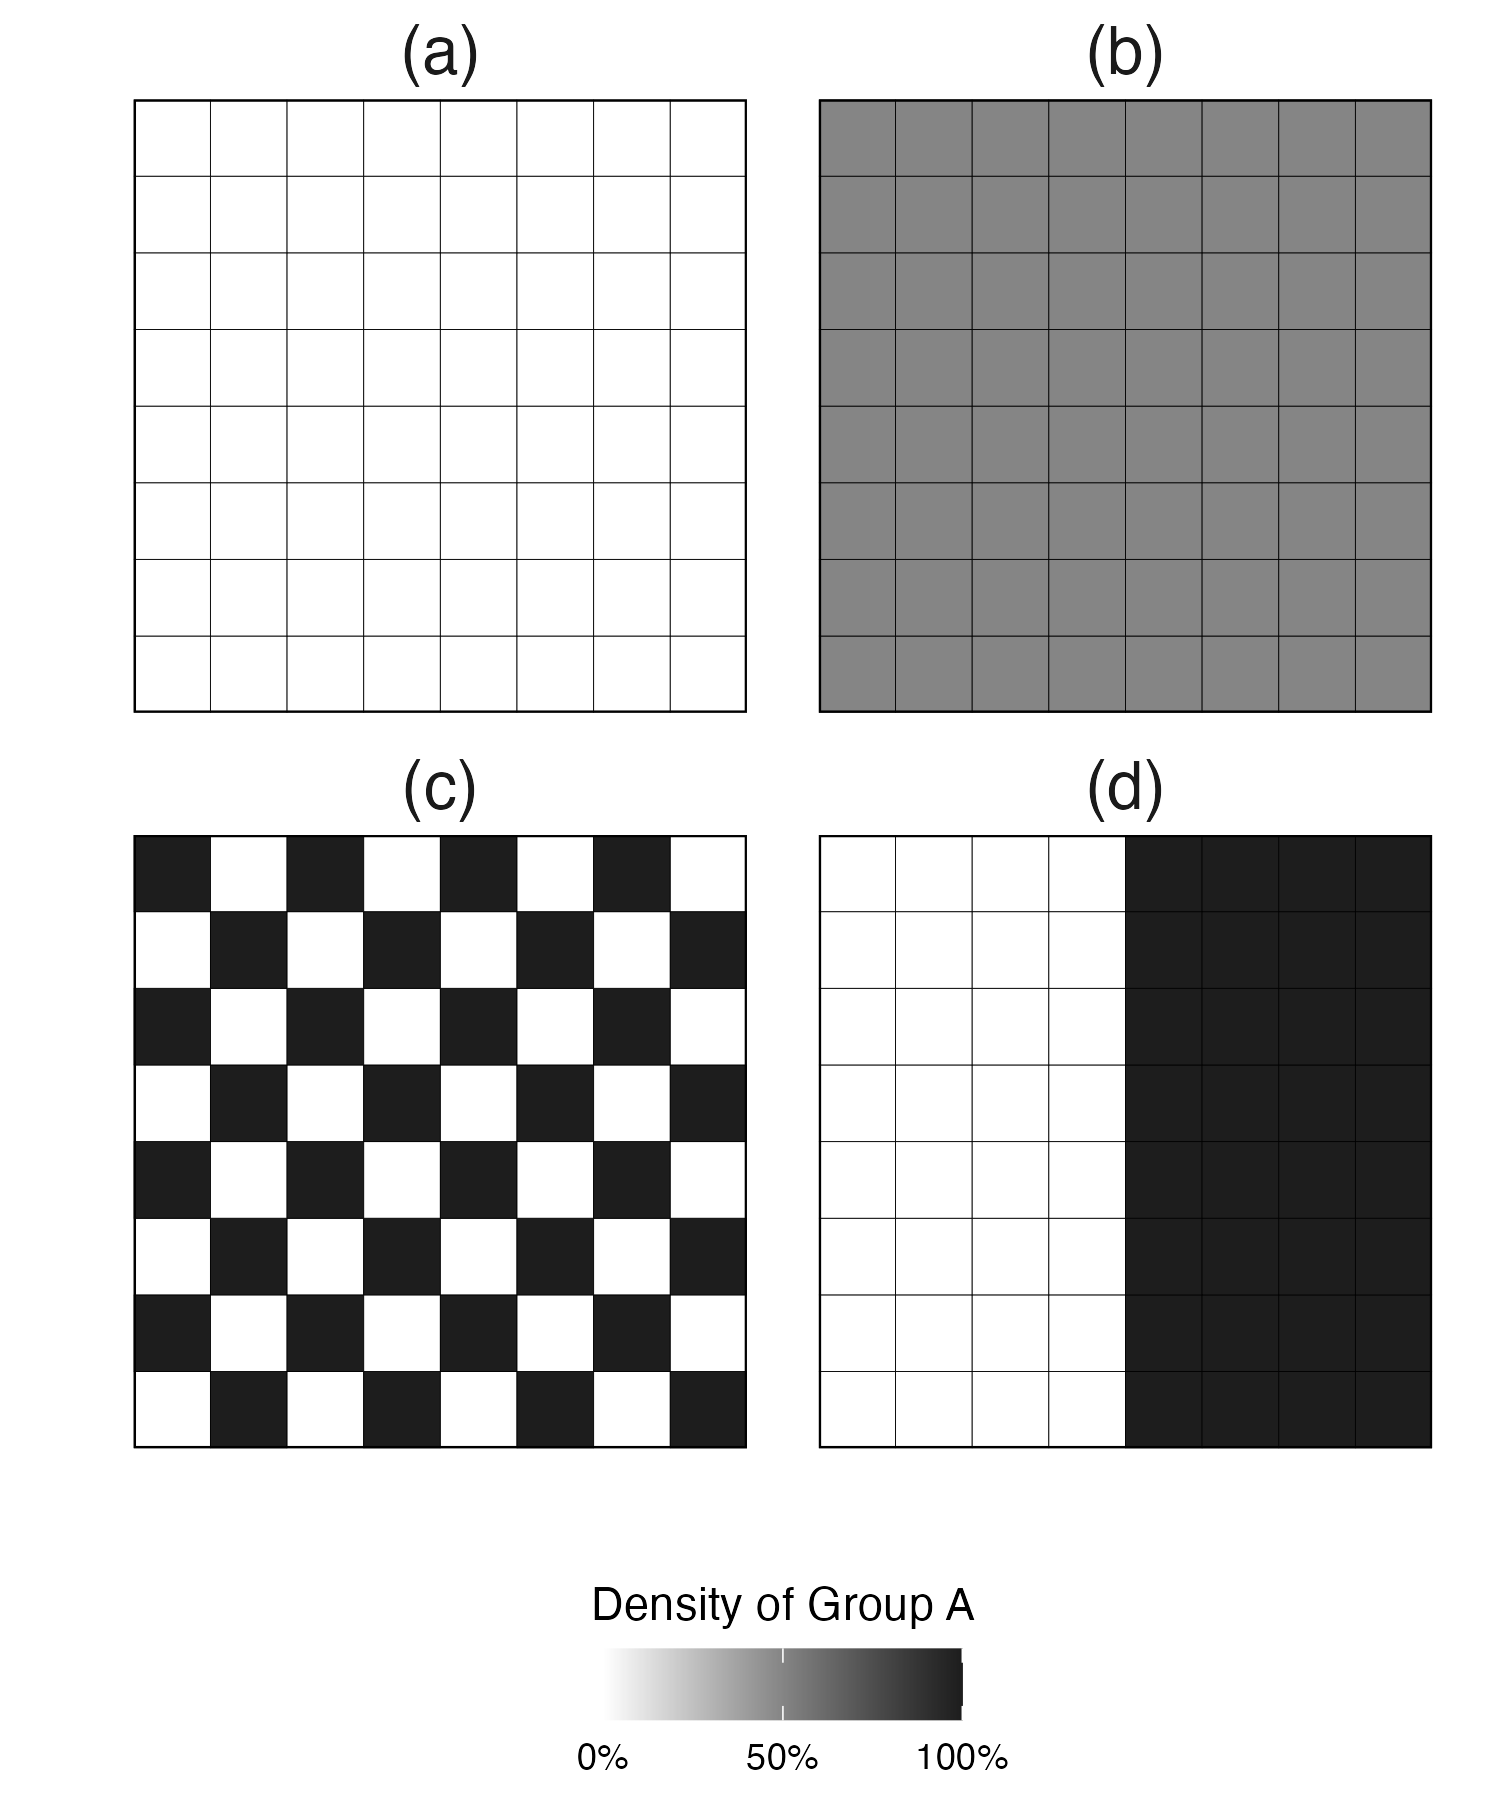
\includegraphics[width=0.5\textwidth]{fig/checkerboards.png}
  \caption{A simple checkerboard pattern.} \label{fig:checkerboard}
\end{figure}



\subsection*{references: use MR numbers!}
There is an absolute maximum of 20 references for any article.  The AMS uses MR style for references. If you are using a BibTeX style
bibliography file (.bib), these will be formatted automatically by this
document. Otherwise, follow the guides below. \textbf{Please also be sure
to include MR numbers, if they exist, for all references listed.}
If you are cutting and pasting your references from MathSciNet, these are
included automatically. Otherwise, please add the MR number as in this one
(from a nice article on Galois theory for quasi-fields \cite{MR0001219}):

\begin{verbatim}
@article {MR0001219,
AUTHOR = {Jacobson, N.},
TITLE = {The fundamental theorem
  of the {G}alois theory for quasi-fields},
JOURNAL = {Ann. of Math. (2)},
FJOURNAL = {Annals of Mathematics.
  Second Series},
VOLUME = {41},
YEAR = {1940},
PAGES = {1--7},
ISSN = {0003-486X},
MRCLASS = {09.1X},
MRNUMBER = {0001219},
MRREVIEWER = {R. Brauer},
DOI = {10.2307/1968817},
URL = {http://doi-org/10.2307/1968817},
}
\end{verbatim}

\subsection*{I can't find an MR number?!}

If you don't have an MR number, the DOI and URL fields are also very useful for
the Notices staff. The URL field can contain any link which will take the
user to the paper. For the above paper, for example, we could have used:
\begin{verbatim}
URL = {http://www.jstor.org/stable/1968817}
\end{verbatim}

\subsection*{References won't compile}

If you don't see a reference at the bottom of this document when you compile, 
then include the extension .bib in the parameter for the \verb!\bibliography!
command.

%\bibliographystyle{foo}
\bibliography{refs}

\end{document}

%%% Local Variables:
%%% mode: latex
%%% TeX-master: t
%%% End:
